\begin{enumerate}[label=\thesubsection.\arabic*.,ref=\thesubsection.\theenumi]
\numberwithin{equation}{enumi}

\item
For a unity feedback system shown in  Fig.  \ref{fig:ee18btech11038_flow}, having transfer function given below in eq \ref{eq:ee18btech11038_tf}.  Design the value of gain K for $\brak{i}$ a gain margin of 38 dB. $\brak{ii}$ Phase margin of 40\degree. $\brak{iii}$ to yield maximum peak overshoot of 20 percent for a step input.

\begin{figure}[!ht]
	\begin{center}
		
		\resizebox{\columnwidth}{!}{%\begin{figure}
\tikzstyle{block} = [draw, fill=blue!20, rectangle, 
    minimum height=1cm, minimum width=1cm]
\tikzstyle{sum} = [draw, fill=blue!20, circle, node distance=1cm]
\tikzstyle{input} = [coordinate]
\tikzstyle{output} = [coordinate]
\tikzstyle{pinstyle} = [pin edge={to-,thin,black}]

% The block diagram code is probably more verbose than necessary
\begin{tikzpicture}[auto, node distance=2cm,>=latex']
    % We start by placing the blocks
    \node [input, name=input] {X(s)};
    \node [sum, right of=input] (sum) {};
    
    \node [block, right of=sum] (system) {$G(s)$ };
   
    % We draw an edge between the controller and system block to 
    % calculate the coordinate u. We need it to place the measurement block. 
    
    \node [output, right of=system] (output) {};
    \node [block, below of=system] (measurements) {1};

    % Once the nodes are placed, connecting them is easy. 
    \draw [draw,->] (input) -- node {$U(s)$} (sum);
    \draw [->] (sum) -- node {} (system);
    \draw [->] (system) -- node [name=y] {$Y(s)$}(output);
    \draw [->] (y) |- (measurements);
    \draw [->] (measurements) -| node[pos=0.99] {$-$} 
        node [near end] {} (sum);
\end{tikzpicture}
%\end{figure}}
	\end{center}
\caption{}
\label{fig:ee18btech11038_flow}
\end{figure}

\begin{align}
\label{eq:ee18btech11038_tf}
G\brak{s} &= \frac{K\brak{s+2}}{s\brak{s+3}\brak{s+4}\brak{s+5}}
\end{align}
\solution 

\begin{align}
\label{eq:ee18btech11038_TF(s)}
G\brak{s}H\brak{s} &=\frac{K\brak{s+2}}{s\brak{s+3}\brak{s+4}\brak{s+5}}
\end{align}
Name-
\begin{align}
\label{eq:ee18btech11038_T(s)}
T\brak{s} &= \frac{\brak{s+2}}{s\brak{s+3}\brak{s+4}\brak{s+5}}
\end{align}
Assuming positive value of K. Gain -
\begin{align}
\label{eq:ee18btech11038_gain}
      = 20log\brak{\abs{G\brak{s}H\brak{s}}}
    \\ \implies 20log\brak{K} +20log\abs{T\brak{s}}
\end{align}
Phase-
\begin{align}
\label{eq:ee18btech11038_phase}
      = \angle{G\brak{s}H\brak{s}}
    \\ \implies \angle{T\brak{s}}
\end{align}
 Thus value of K has - a) no effect on phase. b) linear effect on gain.




\item $\brak{i}$ Given gain = 38dB
\\
\solution The following code generates Bode plot of $T\brak{s}$ as shown in Fig \ref{fig:ee18btech11038_a}

\begin{lstlisting}
codes/ee18btech11038_a.py
\end{lstlisting}

\begin{figure}[!ht]
\centering
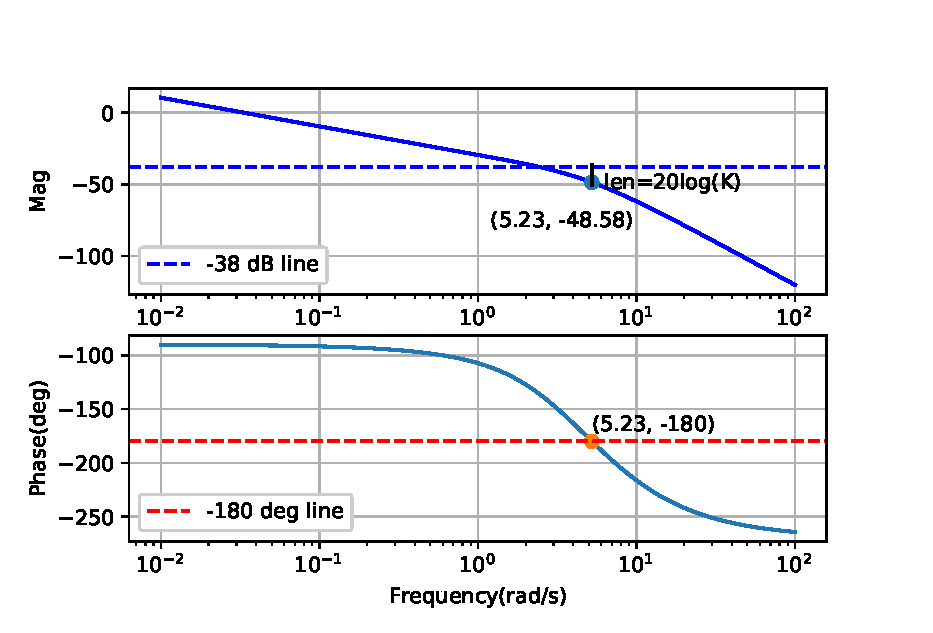
\includegraphics[width=\columnwidth]{./figs/ee18btech11038_a.eps}
\caption{Bode Plot of $T\brak{s}$}
\label{fig:ee18btech11038_a}
\end{figure}
Fig \ref{fig:ee18btech11038_a} shows how much the gain graph be slided to get -38 dB gain at $\omega_{pc}$.
From the graph $K = 3.38$
\item Verify by substituting value of K obtained above. 
\\
\solution The following code generates Fig \ref{fig:ee18btech11038_vera}.

\begin{lstlisting}
codes/ee18btech11038_vera.py
\end{lstlisting}

\begin{figure}[!h]
\centering
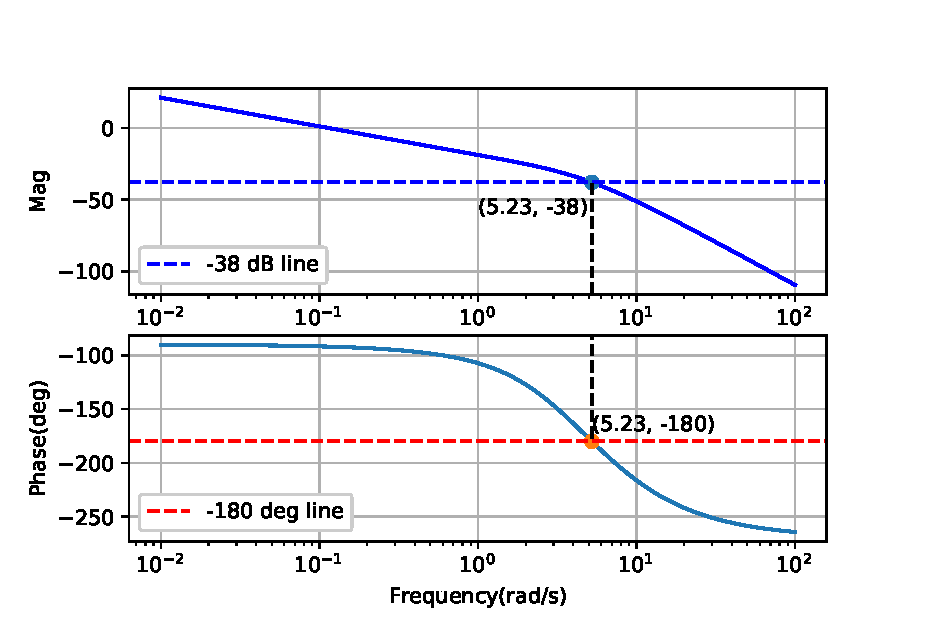
\includegraphics[width=\columnwidth]{./figs/ee18btech11038_vera.eps}
\caption{Bode Plot of $G\brak{s}$ with $K=3.38$ }
\label{fig:ee18btech11038_vera}
\end{figure}

\item $\brak{i}$ Given PM = 40\degree
\\
\solution
\begin{align}
    phase\; at\; \omega_{gc} = -180\degree + PM
    \\
    \implies -140\degree
\end{align}
The following code generates Bode plot of $T\brak{s}$ to obtain $\omega_{gc}$ as shown in Fig \ref{fig:ee18btech11038_b}

\begin{lstlisting}
codes/ee18btech11038_b.py
\end{lstlisting}

\begin{figure}[!ht]
\centering
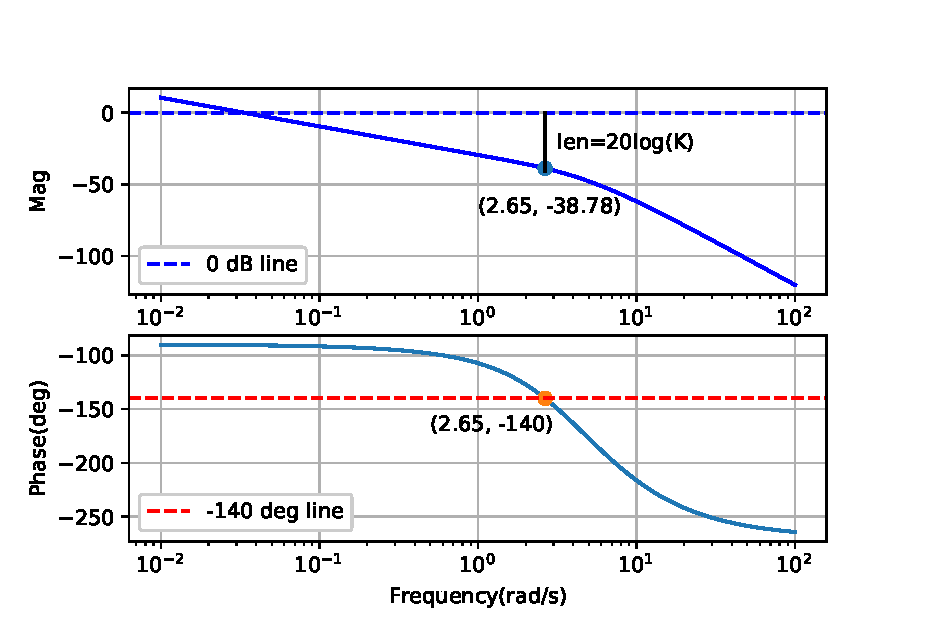
\includegraphics[width=\columnwidth]{./figs/ee18btech11038_b.eps}
\caption{Bode Plot of $T\brak{s}$}
\label{fig:ee18btech11038_b}
\end{figure}
Fig \ref{fig:ee18btech11038_b} shows how much the gain graph be slided to get 0 dB gain at $\omega_{gc}$.
From the graph $K =86.87$ 
\item Verify by substituting value of K obtained above. 
\\
\solution The following code generates Fig \ref{fig:ee18btech11038_verb}.

\begin{lstlisting}
codes/ee18btech11038_verb.py
\end{lstlisting}

\begin{figure}[!h]
\centering
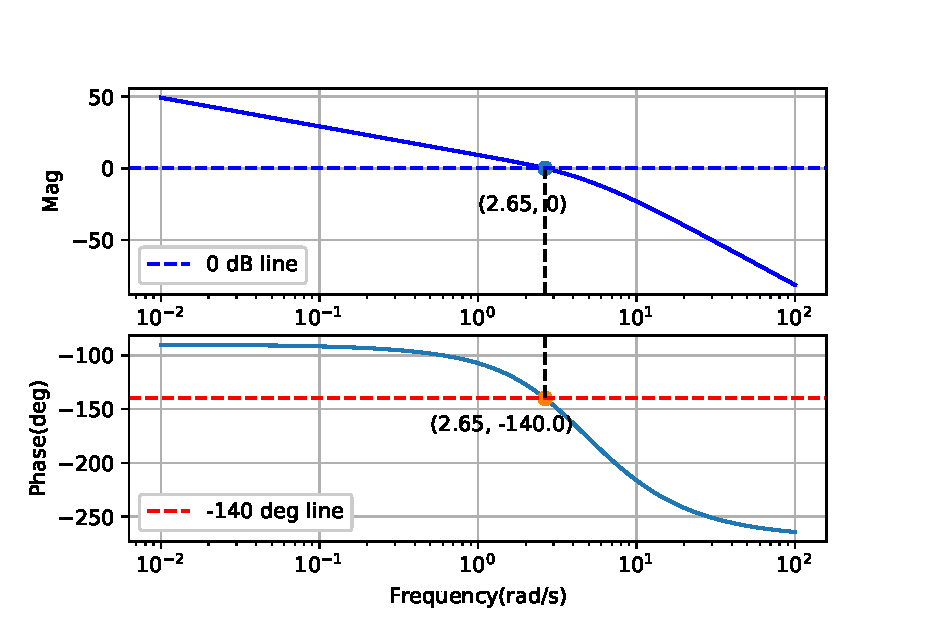
\includegraphics[width=\columnwidth]{./figs/ee18btech11038_verb.eps}
\caption{Bode Plot of $G\brak{s}$ with $K= 86.87$}
\label{fig:ee18btech11038_verb}
\end{figure}

\item $\brak{iii}$ 20 percent peak overshoot in step response.
\\
\solution 
\begin{align}
    \frac{G\brak{s}}{1+G\brak{s}} \quad \quad \quad\quad\quad
    \\
    \implies \frac{K\brak{s+2}}{s^4 + 12s^3 + 47s^2 + \brak{60+K}s + 2K} &= C\brak{s}
\end{align}
Step response-
\begin{align}
    \frac{K\brak{s+2}}{\brak{s}[s^4 + 12s^3 + 47s^2 + \brak{60+K}s + 2K]}
\end{align}
By final value theorem, steady state value-

\begin{align}
    \lim_{s \to 0} sC\brak{s} = \lim_{t \to \infty} c\brak{t} = 1
\end{align}
So the value at peak should be 1.2.
Now it is extremely difficult to find K  from the given data. Routh Hurwitz criteria only reveals that positive $K<156$.
Since it a fourth order system, there exist no explicit formula for peak time. Thus, trying a random value of K under the bound, then taking inverse Laplace and differentiating to get peak time and thus overshoot, is the only method that remains. Using trial and error K = 69.2 and Tpeak =1.19s

 \item Verify by substituting value of K. 
\\
\solution The following code generates Fig \ref{fig:ee18btech11038_os}.

\begin{lstlisting}
codes/ee18btech11038_os.py
\end{lstlisting}

\begin{figure}[!h]
\centering
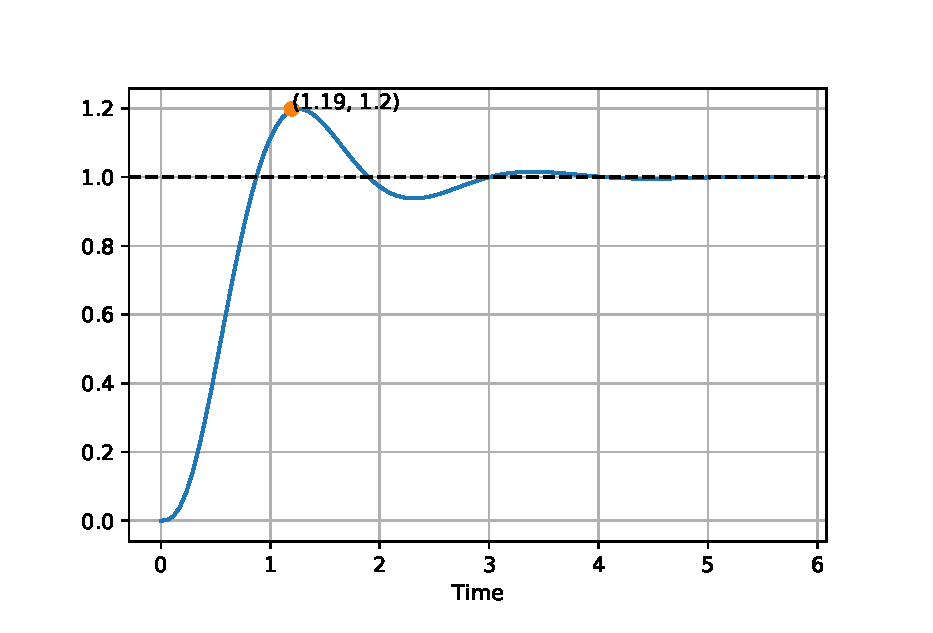
\includegraphics[width=\columnwidth]{./figs/ee18btech11038_os.eps}
\caption{Step Response of the sysytem for K = 69.2}
\label{fig:ee18btech11038_os}
\end{figure}
\end{enumerate}